\documentclass[a4paper, 12pt]{article}

% Packages
\usepackage[utf8]{inputenc} % UTF-8 encoding
\usepackage[T1]{fontenc}    % Font encoding
\usepackage[english]{babel}  % Language
\usepackage{graphicx}       % For including images
\usepackage{amsmath}        % Math packages
\usepackage{amsfonts}
\usepackage{amssymb}
\usepackage{natbib}         % Bibliography package
\usepackage{url}            % URL formatting
\usepackage{hyperref}       % Hyperlinks
\usepackage{geometry}       % Adjust page margins
\usepackage{setspace}       % Adjust line spacing

\graphicspath{{Images/}}

% Title and Author
\title{Survey of Strontium Isotope Analysis in Archeolgical Research of Ancient Egypt}
\author{Jaxon Lee}
\date{\today}

\begin{document}

\maketitle

\begin{abstract}
    This paper explores the pivotal role of strontium isotope analysis in reshaping our understanding of Ancient Egyptian history. It delves into the methodology, challenges, and advancements in this analytical approach, emphasizing its ability to discern geographic origins and trace human movements.
\end{abstract}

\section{Introduction}
The exploration of Ancient Egyptian civilization has been significantly enhanced by
advancements in analytical techniques, particularly the application of strontium
isotope analysis. This paper navigates the transformative role of strontium isotope
studies in augmenting our comprehension of Ancient Egyptian history.

Archaeologists routinely unearth human skeletal remains, and one valuable tool for
elucidating more about them is isotope analysis. This involves investigating the
levels of various elements such as oxygen, carbon, or strontium using chemistry.
Strontium isotope analysis, in particular, proves indispensable for archaeologists
as it facilitates an understanding of the geographic movement of humans and animals.

Over the last decade, strontium isotope analysis has gained substantial momentum,
propelled by advancements in measuring technology \citep{holt2021}. While a
comprehensive study of strontium isotope analysis and its broad application to archaeology
exceeds the scope of this paper, my focus centers on its relevance to archaeological
research in Ancient Egypt. This choice is driven by the intriguing application of
strontium isotope analysis to Egyptian mummies.

Within the confines of Ancient Egypt, a rich array of questions has emerged, leading
to insightful revelations through strontium isotope analysis. This paper aims to
illuminate how strontium isotope analysis functions, its primary use cases, and several
compelling case studies that leverage its potential.

\section{Strontium Isotope Analysis}
\subsection{Overview}
\begin{figure}[htbp]
    \centering
    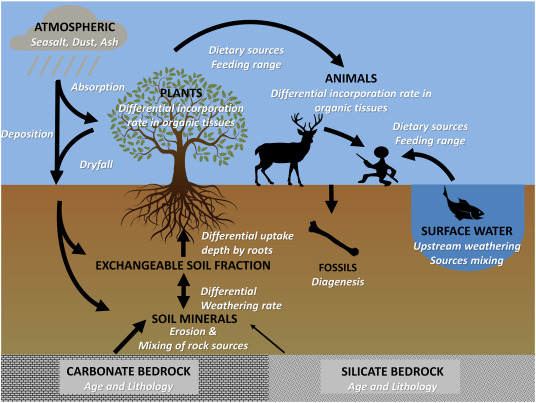
\includegraphics[width=0.8\textwidth]{strontium_process.jpg}
    \caption{A depiction of how strontium goes from bedrock into the ecosystem, where every arrow
        represents the movement of strontium \citep{bataille2020}.}
    \label{fig:strontium_process}
\end{figure}

Strontium is an element, which occurs naturally at varying concentrations in rock formations.
Strontium gets into the water stream through erosion and eventually is inadvetently consumed by plants and animals in trace amounts \citep{bartelink2019}.
Eventually, when humans or animals inevitably consume plants, water, or other animals,
a small amount of strontium gets into their bones and tissue. Notably, although the amount is trace, the
ratio of strontium stays constant throughout all these processes since there is no "isotopic fractionation" \citep{bartelink2019}.
Thus, measuring strontium in bones or tissue gives a picture of where humans or animals source their food and water.
The process by which strontrium goes through an ecosystem is in Figure~\ref{fig:strontium_process}.


\subsection{How It Works}

Now, I will describe in detail how archeologists do strontium isotope analysis.
First, an "isotope" is a version of an element with a particular atomic weight,
which is indicated by a superscripted number to the left of the elemental symbol \citep{Meave60_2015}.
For example, one isotope of Oxygen is \textsuperscript{18}O, where 18 represents
the atomic weight of the isotope. There are four possible isotopes of strontium in
nature \citep{holt2021}, but only two are relevant to strontium isotope analysis: \textsuperscript{87}Sr and \textsuperscript{86}Sr.
Notably, these isotopes are extremely stable, so they do not react with other elements
and their abundances in the environment will stay constant unless outside forces interfere \citep{Long1998}.

One such outside force is the radioactivity of \textsuperscript{87}Rb, which forms \textsuperscript{87}Sr when it decays. So, the \textsuperscript{87}Sr concentration in a substance
will increase over time depending on the initial concentration of \textsuperscript{87}Rb.
\textsuperscript{87}Rb has a half-life of 48.8 billion years, so it takes billions of years
for \textsuperscript{87}Rb to fully decay into \textsuperscript{87}Sr; as a result, \textsuperscript{87}Rb will always
have a small but measurable effect on the \textsuperscript{87}Sr levels of the substance it is in.
Thus, the relative concentraion of \textsuperscript{87}Sr / \textsuperscript{86}Sr is constantly increasing.

In contrast with the stable strontium, \textsuperscript{87}Rb varies signifantly across the environment.
This is because of how rocks form; in deep Earth layers, magma mixes and moves constantly, which spreads and changes \textsuperscript{87}Rb concentrations.
In addition, when the magma cools,
\textsuperscript{87}Rb will spread out such that even different parts of the same
rock formation have different \textsuperscript{87}Rb concentrations.

Throughout all of this, \textsuperscript{87}Sr and \textsuperscript{86}Sr concentrations remain
generally constant due to the aformentioned stability and the fact that strontium isotopes
do not fractionate, or separate, at magma tempeartures.
% ^ This might not be right.
Therefore, different rock formations will have different quantities of
\textsuperscript{87}Sr and \textsuperscript{86}Sr depending on where the rock formed,
when it formed, and the initial concentrations of \textsuperscript{87}Rb, \textsuperscript{87}Sr, and \textsuperscript{86}Sr \citep{Long1998}.

For the purposes of archeology, we can assume that every rock has a random, unique
concentration of \textsuperscript{87}Sr and \textsuperscript{86}Sr. As stated previosuly,
the concentrations of these two values eventually travel through the ecosystem to all nearby
plants and animals. Since the exact concentrations may get diluted, archeologists often
measure the ratio of \textsuperscript{87}Sr / \textsuperscript{86}Sr since this
remains constant through the strontium transfer process \citep{bartelink2019}.

% TODO: Discuss how its measured
Archeologists can use a mass spectrometer to determine this ratio \citep{Long1998}.

In summary, \textsuperscript{87}Sr / \textsuperscript{86}Sr ratios can serve as a
"fingerprint" for identifying geographic areas since they vary greatly
across the environment. This is useful for archeologists because strontium isotope ratios
can be measured in organic material to get an idea of where the tissue was when it formed.
Also, strontium isotopes are stable once formed. Thus, measuring strontium isotope ratios is
desirable because there are essentially no unpredictable
factors that can affect the measurement.

% \citep{holt2021} https://www.sciencedirect.com/science/article/pii/S0012825221000933?casa_token=FLhhJysXAz4AAAAA:VTVcEUD71ZsaI0siB8F-2VvDoI03s2EC1zN-20NrsRFemTiffkhW5X0yz_8Iv1-NxARwqwhL6vE
% \citep{crowley2017} https://onlinelibrary.wiley.com/doi/full/10.1111/brv.12217?casa_token=fzF_HvyFA3EAAAAA%3ACWLmQaH1S_B4GXOgCmSZJYwQr-NNwC4iUxP1kPFA8Tw05-d65rejwmCkDgQ3itV6APu8LbHSWdOOcuCY
% [4] https://link.springer.com/article/10.1007/BF01100444
% \citep{kozieradzkaogunmakin2021} https://brill.com/display/book/9789004433755/BP000007.xml
% \citep{barfod2020} https://www.nature.com/articles/s41598-020-68089-w
% \citep{kamenov2014} https://anthrosource.onlinelibrary.wiley.com/doi/full/10.1111/napa.12048?casa_token=rWbuuiJYOvIAAAAA%3AcVqQVNRLjm3TVnsmeJyJ4JxPgPuKJeEbIRmWrQ_lV49lztX-XaL17cd9bn3bxJeketNDv0zj1b2jcWRT
% \citep{lazzerini2021} https://www.nature.com/articles/s41598-021-81923-z

\subsection{Purpose}
The main use of strontium isotope analysis in Egyptian archeology is to understand
"provenenance," or place of origin. Since most bones remold over time, measuring their
strontium levels gives insight into the last 7-10
years of a person's life. Measuring the strontium of human hair can tell where someone
took residence immediately prior to death \citep{kamenov2014}. Although this is trivially useful for fields such as forensics \citep{kamenov2014},
archeologists usually have a good idea of where a person lived before they died
since people are usually buried where they lived. However, since tooth enamel
forms during childhood and does not change, measuring it can give the general location
that the person lived in during their tooth formation, i.e., when they were a child
\citep*{holt2021,kozieradzkaogunmakin2021,lazzerini2021}. Thus, archeologists can
identify the provenance of skeletal remains they dig up, so long as they have access
to tooth enamel samples. Other isotopes can be analyzed to similar ends, but
strontium is particularly useful because of the aformentioned stability. There are only
a few factors that can affect strontium isotope ratios, which aids analysis.

\subsection{Isoscapes}
% How they make isoscapes
In order for strontium isotope measurements of organic tissue to be useful, archeologists need to know
which ratios correspond with which places.
So, archeologists create "isoscapes," which are maps of the expected
\textsuperscript{87}Sr / \textsuperscript{86}Sr ratios
of samples in various geographic regions. This creates a baseline that other archeologists
can compare against when doing strontium analyses.

I will discuss the three main approaches for creating an isoscape: domain mapping,
contour mapping, and machine learning \citep{holt2021}. I will also go over their
strengths and weaknesses.
\subsubsection{Domain Mapping}
\begin{figure}[htbp]
    \centering
    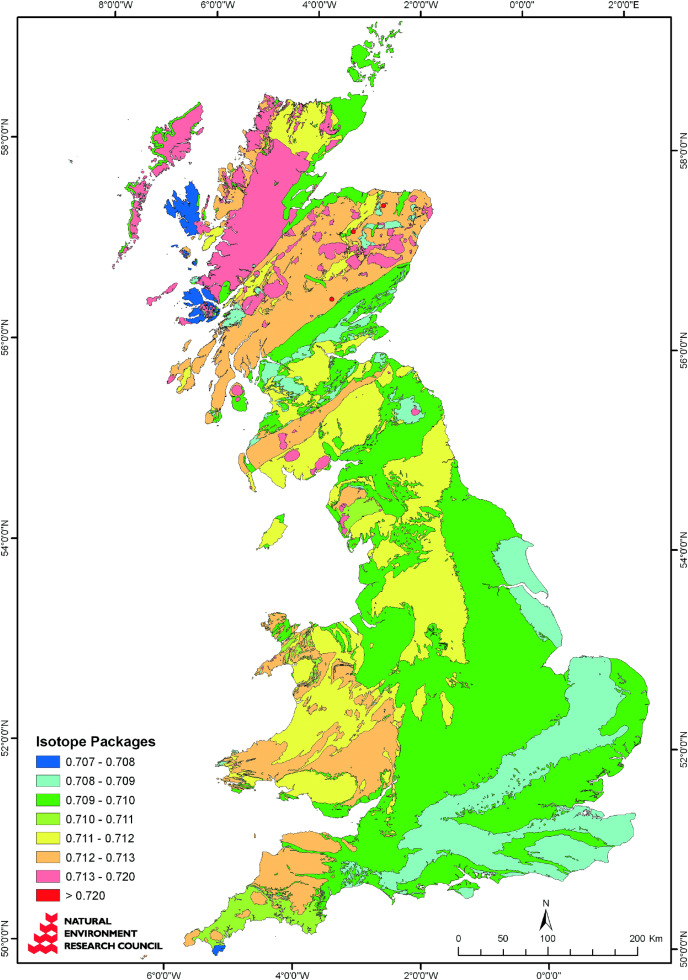
\includegraphics[width=0.45\textwidth]{domain_mapping.jpg}
    \caption{A domain map of Great Britain \citep{evans2010}.}
    \label{fig:domain_mapping}
\end{figure}
To make a domain map, researchers sample the strontium isotope ratios of
various locations, plot the results on a map, and then group similar results
together by hand into "domains." Usually, researchers take multiple samples of
in each region and average them to ensure outliers do not throw off the results.
This is the simplest approach to creating an isoscape, but it is expensive due to the number
of samples one needs to collect to gain a resolution comparably to other methods. For this reason,
domains usually also have low resolution due to limited time and money to sample regions.
Despite this, domain mapping is generally considered the best isoscape approach by researchers
now \citep{holt2021}.
An example of a domain map can be seen in Figure~\ref{fig:domain_mapping}.


\begin{center}
    \begin{tabular}{||c | c||}
        \hline
        Advantages            & Disadvantages            \\ [0.5ex]
        \hline\hline
        Easy to make          & Imprecise                \\
        \hline
        Simple to interpret   & Requires lots of samples \\
        \hline
        Fast to use once made & Expensive                \\
        \hline
                              & Time consuming           \\ [1ex]
        \hline
    \end{tabular}
\end{center}

\subsubsection{Contour Mapping}
\begin{figure}[htbp]
    \centering
    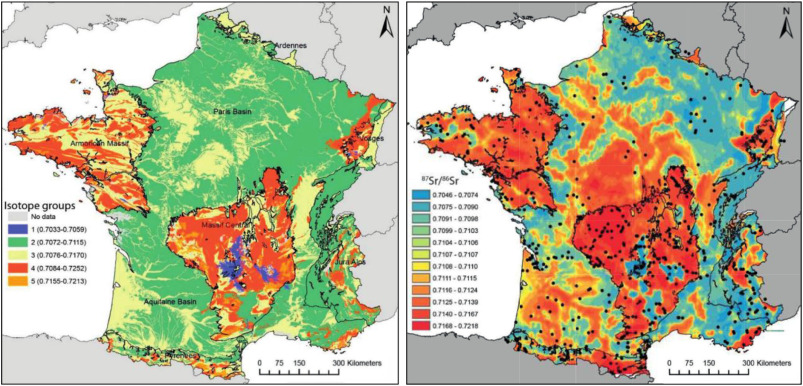
\includegraphics[width=0.9\textwidth]{contour_mapping.jpg}
    \caption{A domain map of France (left) versus a contour map of France (right) \citep{willmes2018}}
    \label{fig:contour_mapping}
\end{figure}

For contour maps, researchers take \textsuperscript{87}Sr / \textsuperscript{86}Sr
samples just as they would for domain mapping, but they use statistics to extrapolate
strontium isotope ratios between the sampling areas instead of grouping similar results
by hand. This can greatly increase resolution and reduce the number of samples needed to make a full isoscape. Some statistical
methods that researchers use for contour mapping are inverse distance weighting, ordinary kiging, empirical bayesian kirigin,
and cokroing \citep{holt2021}. Unfortunately, researchers agree that this approach is ineffective
because strontium ratios do not gradually change between sampling areas. In reality,
they have sharp drop-offs due to the underlying rock formations \citep{holt2021}, which
no statistical method can predict. A contour map is shown along with a domain map of the same
area in Figure~\ref{fig:contour_mapping}. As can be seen, the contour map has more
fluid boundaries and twice as much resolution when compared with the domain map.

\begin{center}
    \begin{tabular}{||c | c||}
        \hline
        Advantages             & Disadvantages                       \\ [0.5ex]
        \hline\hline
        High resolution        & Generally inaccurate                \\
        \hline
        Can give exact results & Can generate impossible results     \\
        \hline
        Relatively cheap       & Unreliable                          \\
        \hline
                               & Can not predict sharp ratio cutoffs \\[1ex]
        \hline
    \end{tabular}
\end{center}

\subsubsection{Machine Learning}
\begin{figure}[htbp]
    \centering
    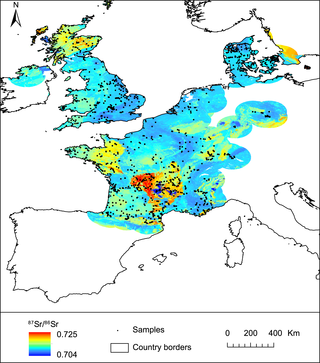
\includegraphics[width=0.5\textwidth]{machine_learning_isoscape.png}
    \caption{A machine learning-based isoscape of Western Europe \citep{bataille2018}.}
    \label{fig:machine_learning}
\end{figure}
For machine learning-based approaches, researchers use algorithms
that learn how to predict
strontium isotope ratios based on existing strontium samples, models of natural processes such as chemical weathering, and
environmental data like geological maps \citep{bataille2018}.
One example of a machine learning algorithm used for this purpose is random forest regression
\citep{bataille2018}. Notably, machine learning algorithms are capable of predicting
the sharp drop-offs we expect from strontium ratios in isoscapes, which contrasts
with contour mapping approaches. Furthermore, machine-learning based approaches are
capable of displaying the confidence of a particular measurement or region of
measurements; this allows researchers to gauge how much they should trust a measurement
and also give ideas on where to sample next to improve the isoscape.
Early results show these models to be extremely effective at producing accurate
isoscapes. However, these algorithms are complex, are still being proven, and have
yet to be applied globally. An example of an isoscape generated by random forest
regression can be seen in Figure~\ref{fig:machine_learning}.

\begin{center}
    \begin{tabular}{||c | c||}
        \hline
        Advantages                              & Disadvantages                  \\ [0.5ex]
        \hline\hline
        High resolution                         & Complicated to make            \\
        \hline
        Can give exact results                  & Computationally intensive      \\
        \hline
        Extremely accurate                      & Not fully fleshed out          \\
        \hline
        Gives prediction confidence             & Needs lots of extra data       \\
        \hline
        Additional variables can be factored in & Limited applications presently \\[1ex]
        \hline
    \end{tabular}
\end{center}


\subsection{History}
I will briefly explain how strontium isotope analysis came to exist, major advancements,
and where it is trending towards now. Originally, strontium isotope analysis was used simply to age rocks, study erosion, and
find the source of rivers \citep*{moorbath1965, crowley2017}. Around the late 1980s and early 1990s, archeologists theorized
that strontium isotope analysis of tooth enamel could be used to learn where a human originated \citep{crowley2017}. This spawned
a flood of studies to prove its viability and test its limitations \citep{crowley2017}.
Since then, archeologists have increasingly used strontium isotope analysis to answer
questions of human provenance. Recently, there has been an explosion of strontium
isotope analysis research \citep{crowley2017}; scientific
breakthroughs such as high performance laser ablation and multicollector inductively coupled
plasma mass sepctrometry and increasing availability of high-quality isoscapes \citep{crowley2017}
have made strontium isotope analysis more accessible and more effective \citep{holt2021}.
According to \cite{holt2021}, the main focus of strontium research now is creating new isoscapes
and refining existing ones. The advent of machine learning-based approaches to isoscapes
is particularly interesting as it could drastically increase the resolution of isoscape
baselines and potentially allow more specific regional identification from strontium
isotope analysis.
% History
% - Age of rock
% - Originally about rock erosion and where Sr came from regarding rivers \citep{crowley2017}
% - Late 80s/early 90s-- first uses of Sr to detect where person came from. Lots of studies to prove that it could viably be used in this way\citep{crowley2017}
% - Ramping up in last decade \citep{crowley2017}
% - A lot of recent advancements  \citep{holt2021}
% -> "high performance laser ablation" and "multicollector inductively coupled plasma mass spectrometry"
% - Current goal- isoscapes \citep{holt2021}




% Limitations
% - Often is not precise to conclusively answer questions by itself. Best used in combination with other methods, such as analyzing other isotopes. \citep{holt2021}
% - Expensive \citep{crowley2017}
\subsection{Limitations}
The main weaknesses of strontium isotope analysis are accuracy, precision, and cost.
\subsubsection{Accuracy}
Strontium isotope analysis can sometimes be inaccurate. A person consistently moving
across areas during childhood can make their tooth enamel strontium ratios indiscernible.
But, it is generally a reasonable assumption that people did not travel during childhood
in the context of archeology since travel was historically harder than today and children need time to grow.
Also, people might source their food and water from a different geographic region from where
they lived, which could throw off results.
This is further complicated by plant consumption disproportionately affecting strontium ratios \citep{price2006}.
So, even if the majority of a
person's diet consisted of local food and water, a relatively
small amount of non-local farm products could give a false-negative on a locality test.
But, if one understands what historical people ate and where they got their food,
one can account for these dietary effects in one's strontium isotope analysis.



\subsubsection{Precision}
Strontium isotope analysis can give results that are too broad. In many parts of the world, isoscapes are not
refined.
% Maybe add source for thuis ^
So, strontium measurements only give a general region of provenance, which is sometimes insufficient to answer a research question.
% This is why "local vs non-local" questions are common
However, this can be alleviated by combining strontium isotope analysis with other tools,
such as analyzing isotopes of \textsuperscript{13}C, \textsuperscript{18}O, and \textsuperscript{34}S
to understand diet, climate, and likely distance to a water source respectively \citep{madgwick2019}.
If different sources of data support the same conclusion, then that conclusion
is likely true.

\subsubsection{Price}
Strontium isotope analysis is expensive \citep{holt2021}. It involves highly specialized tools along
with expertise in chemistry to operate them. Furthermore, researchers must take many samples to get
meaningful results. Although there is no immediate solution to this, the best approach
is to apply strontium isotope analysis only where needed and leverage its results
as much as possible. However, as technology improves, strontium
isotope analysis will inevitably get cheaper and more effective, so I am hopeful
for the future of strontium isotope analysis.


\section{Use Cases}
In this section, I will discuss how
archeologists apply strontium isotope analysis, then I will describe use cases beyond archeology.

\subsection{Archeological Use Cases}
\subsubsection{Local vs Non-Local}
Archeologists often measure the ratio of
skeletons in a graveyard that came from the area around the graveyard versus some
far away area \citep{holt2021}. This approach has the advantage of not requiring
a perfect isoscape since any skeleton that does not fall in the range for the specific
area under study may be classified as "non-local" without needing to know exactly where
they came from.

\subsubsection{Animal Origins}
As another extension of provenance study, prehistoric animal fossils can be analyzed
to uncover their place of origin.
% TODO: NEED TO FIND SOURCE THAT DISCUSSES THIS MORE

\subsubsection{Material Origins}
More rarely, archeologists use strontium isotope analysis to determine the origin
of physical artifacts. For example, Gry Brafod et al. concluded that celebrated
clear glass in Roman cities came from Egypt \citep{barfod2020}.
% - "Provenance" - place of origin \citep{holt2021}
% - Preminent goal is to track movement of animals and humans
% - "Local vs non local" \citep{holt2021}
% - Can be used on "ancient organisms" \citep{crowley2017}
% - Origin of glasswork \citep{barfod2020} -- "Alexandrian glass"

\subsubsection{Crops}
Just as human and animals intake the strontium ratios of their environment, crops
have the same effect. \cite{larsson2020} used strontium isotope analysis to determine the
origins of historic farm produce of Uppåkra in Sweden. They found non-local crops, which
gave insight into trade and movement for the culture under study.
% TODO: Add this 
% Crops - [20]
% [20] https://www.tandfonline.com/doi/full/10.1080/20548923.2020.1840121

\subsubsection{Landscape Use}
Strontium isotope analysis aids in understanding ancient populations' interactions
and utilization of landscapes. This perspective enriches the reconstruction of
ancient societies, offering insights into settlement patterns and land use
practices \citep{crowley2017}.


\subsection{Other Use Cases}
\subsubsection{Forensics}
Strontium isotope analysis can be used to learn more about the body of a recently
deceased victim.
% TODO: Add more to this section.

\subsubsection{Illegally Poached Animals}
Researchers can get an idea of where a poached animal product came from after it
gets to market. This can be useful for finding and shutting down illegal poaching
operations.
% TODO: Add more to this seciton.

\subsubsection{Range of Invasive Species}
Understanding the spread and impact of invasive species in different regions is
essential for assessing environmental changes and human influences. Strontium
isotope analysis helps in mapping the distribution and movement patterns of
invasive species in archaeological contexts \citep{crowley2017}.
% TODO: Improve this




% \subsection{Ancient Habitat Use and Settlement Patterns}
% Strontium isotope analysis unveils insights into settlement patterns. It allows archaeologists to discern whether individuals were indigenous or from other regions, shedding light on migration, resource utilization, and societal dynamics \citep{crowley2017}.

% \subsection{Tracing Animal Origins and Interactions}
% Strontium isotope analysis is instrumental in tracing the origins of diverse animals like anadromous fish and extinct hominins. This exploration offers valuable perspectives on ancient ecosystems, human-animal interactions, and resource exploitation by past societies \citep{crowley2017}.

% \subsection{Unraveling Farm Product Sources}
% By utilizing strontium isotope analysis, researchers uncover the geographic origins of farm products like rice, corn, and medicinal plants. This knowledge contributes to understanding ancient agricultural practices, trade networks, and resource distribution \citep{crowley2017}.

% \subsection{Mapping Migration Routes}
% The application of strontium isotope analysis in mapping migration routes provides critical insights into ancient human mobility, societal exchanges, and the patterns of population movement throughout history \citep{crowley2017}.

% \subsection{Tracing the Origins of Illegally Poached Animals}
% Efforts to combat illegal wildlife trade can be supported through the identification of regions from which poached animals originate using strontium isotope analysis \citep{crowley2017}.

% \subsection{Mapping the Range of Invasive Species}
% Understanding the spread and impact of invasive species in different regions is essential for assessing environmental changes and human influences. Strontium isotope analysis helps in mapping the distribution and movement patterns of invasive species in archaeological contexts \citep{crowley2017}.

% \subsection{Comprehending Landscape Use}
% Strontium isotope analysis aids in understanding ancient populations' interactions and utilization of landscapes. This perspective enriches the reconstruction of ancient societies, offering insights into settlement patterns and land use practices \citep{crowley2017}.

% \subsection{Application in Forensic Studies}
% Beyond archaeology, the use of strontium isotope analysis extends to forensic studies, aiding in determining the geographic origins of individuals and supporting forensic investigations \citep{kamenov2014}.

% - Ancient habitat use \citep{crowley2017}
% - Animal origins \citep{crowley2017}
% --> "anadromous fish", "extinct hominins"
% - Farm product sources, like rice, corn, and drugs \citep{crowley2017}
% - Migration routes \citep{crowley2017}
% - Where illegally poached animals came from \citep{crowley2017}
% - Range of invasive species \citep{crowley2017}
% - Understand landscape use \citep{crowley2017}
% - Forensics \citep{kamenov2014}

% I've chosen Ancient Egypt because Sr analysis is particularly easy to apply b/c of mummies.

% [Same 1] https://www.sciencedirect.com/science/article/pii/S0012825221000933?casa_token=H3KiKu8CjckAAAAA:B4tj30AghfGVDqr1qDlsstbfhMKHja2hn4i0s8Iopsn4oVXcOvlsbJpViADpjDOJlWZUdAWuRXo
% \citep{stantis2021} https://link.springer.com/article/10.1007/s12520-021-01344-x
% \citep{weinstein2021} http://eprints.bournemouth.ac.uk/33312/1/17_Stantis_CAENL%209.pdf -- importance of collecting modern samples, combining Sr with other isotope analyis, and building on previous mobility work
% \citep{maaranen2019} http://eprints.bournemouth.ac.uk/33511/1/N.%20Maaranen1_03.10.19.pdf
% \citep{bartelink2019} https://academic.oup.com/fsr/article/4/1/29/6794654

\section{Case Studies}
Now, I will go over three interesting case studies that use strontium isotope analysis in the
hopes that researchers may get ideas on how to apply strontium isotope analysis to
their own work.
\subsection{The Hyksos' Rise to Power}
% Hyksos

\begin{figure}[htbp]
    \centering
    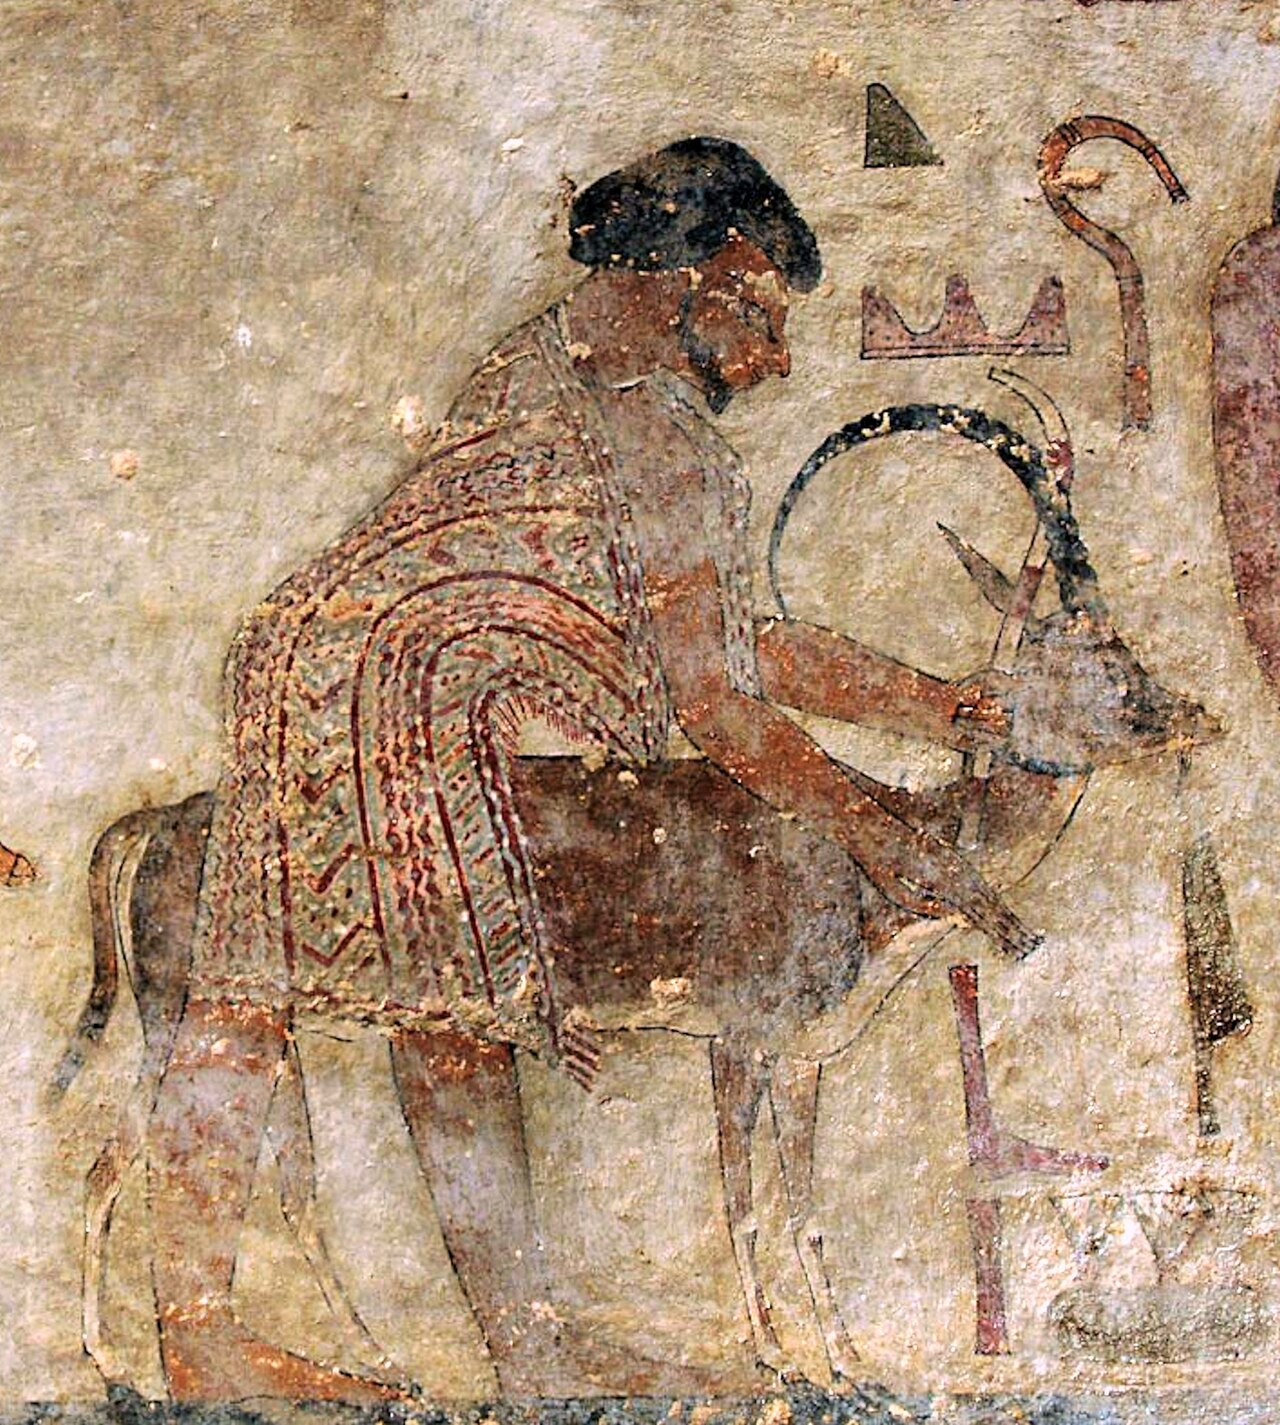
\includegraphics[width=0.5\textwidth]{hyksos_painting.jpg}
    \caption{Egyptian painting of Abisha the Hyksos \citep{wikipediaHyksos}}
    \label{fig:hyksos_painting}
\end{figure}
During the period of 1638 BCE to 1530 BCE, the foreign Hyksos people rose to power
and ruled over Egypt. Unfortunately, little is known about it. What little we do know comes
from a single Egyptian priest named Manetho hundreds of years after the Hyksos were gone,
who claimed that the Hyksos were oppressive rulers who seized power through invasion \citep{stantis2020}.
An ancient picture of a Hyksos ruler is in Figure~\ref{fig:hyksos_painting}. There are a wealth
of resources on applying strontium isotope analysis to the origins of the Hyksos \citep*{stantis2020, stantis2021, weinstein2021, maaranen2019}
I have selected the one I found the most interesting. In a research article from 2020, \cite{stantis2020} challenges this narrative
with evidence gathered with strontium isotope analysis.

The researchers first sought after graves of people who lived during and immediately
before the Hyksos period. They decided to excavate a cemetary in Tell el-Dab'a,
was the capital of the Hyksos kingdom. The cemetary had generations of Egyptians spanning
500 years before and during the Hyksos rule.

Then, the researchers sampled tooth enamel from these skeletons to see if they fell
in the "local" range of strontium ratios. Specifically, they analyzed second permanent molars,
first permanent premolars, and second permanent premolars. 75 skeletons were analyzed,
with half being before the Hyksos rose to power and half being during the Hyksos rule.
The range of strontium ratios that the researchers considered local were
between 0.70761-0.70780, which was based on an isoscape genearted from local animal bones \citep{bournemouth2020}.
%  TODO: check if this is cited correctly

The researchers found that there were numerous non-local people from a wide range
of places across all time periods. About half of all skeletons studied were non-local
according to their strontium isotope ratios, and mot of the non-local people died
during the pre-Hyksos period. Further, there were disproportionately more non-local
women in the researchers' study.

Thus, the researchers concluded that the Hyksos were likely not an invading source
as Manetho asserted. The researchers argue that a more likely explanation was that
the Hyksos arrived centuries before and gradually rose to power. This is supported
by the fact that there were increasing amounts of non-local people before the Hyksos
rose to power. If the Hyksos seized power through invasion, one would expect few non-local
people before Hyksos rule and a large amount of non-local people immediately after they conquered Egypt, which
is not the case. The disproportionate number of non-local women also supports this conclusion
as an invading force would consist of non-local men \citep{stantis2020}.


% - 1638 BC - 1530 BC \citep{stantis2020}
% - Foreign Hysos rise to power
% - Lots of non-local women before Hyksos rule - likely gradual power grab by Hyksos, which contradicts historical narrative \citep{stantis2020}

% - Original narrative: Egyptian priest Manetho-- terrible invasion. But, this was a biased source, albeit the only available source. \citep{stantis2020}
% - Methods:
% --> Excavating various graves
% --> Check tooth enamel (which was formed during childhood) for falling in "local" range of Sr values
% - Conclusions:
% --> Non-local people came from all over
% --> Hyksos were not an invading source. They arrived centuries before and gradually rose to power.
% \citep{stantis2020} https://journals.plos.org/plosone/article?id=10.1371/journal.pone.0235414

% Lots of stuff on the Hyksos. \citep{stantis2020} \citep{stantis2021} \citep{weinstein2021} \citep{maaranen2019}
% - \citep{kozieradzkaogunmakin2021} -- combining Sr analysis with diet analysis to see dietary differences b/w locals and non-locals. No meaningful difference found. Conclusion: confirming previous diet research, can't really use Oxygen analysis to determine local-ness


\subsection{Mummified Birds}
% Mummified Birds
\begin{figure}[htbp]
    \centering
    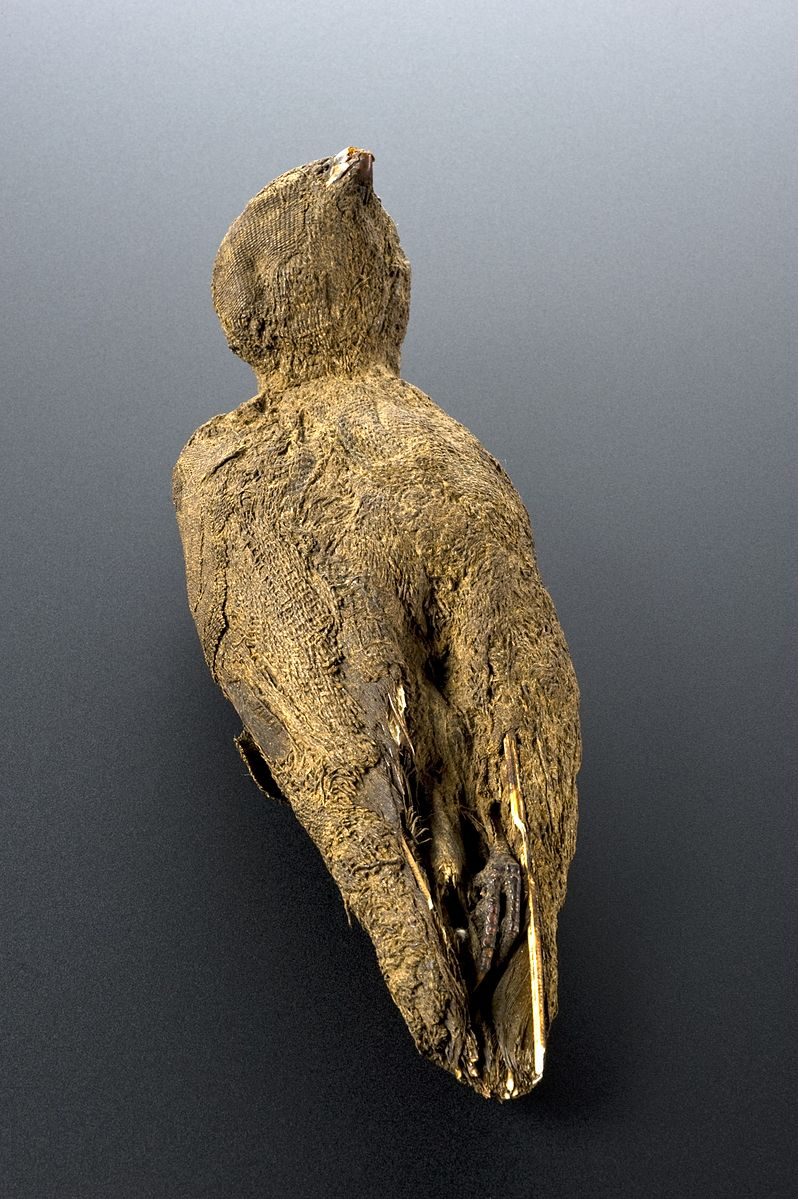
\includegraphics[width=0.35\textwidth]{mummy_bird.jpg}
    \caption{An ancient Egyptian mummified bird \citep{wikipediaBird}}
    \label{fig:mummy_bird}
\end{figure}
In addition to famous human mummies, ancient Egyptians sometimes mummified birds
like ibises or birds of prey. One reason they did this was to honor gods who took
the forms of birds, such as Horus and Thoth. One example of a mummified bird is in Figure~\ref{fig:mummy_bird}.
\cite{linglin2020} asked whether these mummified birds were farmed or hunted in the hopes of understanding
more about ancient Egyptian capabilities, their economy, and potential effects on
the environment.

First, the researchers took bone samples from mummified birds. Samples from major bones were used;
as birds do not have teeth, the researchers could not analyze tooth enamel as they would
with humans or other animals. However, for the purposes of deciding whether the birds
were farmed or hunted, the major bones are sufficient. If the bird was cultivated by the
Egyptians, it would have spent its whole life in the local area, whereas a wild bird
that was caught shortly before mummification would have spent most of its life outside
of the local area.

Then, the researchers combined a few isotopic analyses, including one of strontium ratios.
They determined that the isotope composition likely was not changed during the mummification
procecss or in the time between it being preserved and sampled since the birds were not
buried in potential strontium-leaching ground nor did they have unusual levels
of nitrogen, carbon, or sulfur in their feathers.


They found that most of the ibises were local, but the birds of prey were non-local.
Ibises had \textsuperscript{87}Sr / \textsuperscript{86}Sr ratios consistent
as well as oxygen levels with the local environment. This would support the theory that
ibises were farmed by the Egyptians. However, an analysis of carbon isotopes revealed
significantly higher variance when compared with that of ancient Egyptians. If the ibises
were farmed, they would have a similar or lower variability in carbon compositions, if we
accept that farmed animals would be fed a similar or lower diversity of food compared to
their owners. Also, the ibises did not show substantial genetic overlap as was found in a previous study \citep{wasef2019}, which
further prejiduces the theory that ibises were farmed. However, the researchers concede
that one possible explanation is that ibises were captured and held until they were
needed as an offering.
For the birds of prey, the strontium ratios, when combined with \textsuperscript{18}O analysis, clearly
showed that they did not spend significant time around where they
were mummified.

The researchers thus concluded that the ibises and birds of prey were wild, although
ibises may have been held briefly in captivity before their sacrifice. This could indicate
that ancient Egyptians could not farm ibises and birds of prey, or perhaps that
it was not needed. Further, one can assume there was not a wide-scale bird trade. And,
the fact that the birds were likely hunted means that there could have been an effect
on the bird population levels, although the extent of this effect was not discussed
in the research article.



% - Where ancient Egyptian mummified birds came from
% - Farmed vs hunted -- capabilities, economy, and effect on environment
% - Some bird gods like Horus and Thoth
% - Methods:
% --> Take bone samples from birds
% --> Combination of lots of isotope analyses, including Sr
% - Results:
% --> 8/11 ibises local, birds of prey were not local
% - Conclusions:
% --> ibises and birds of prey were wild-- they all moved a good deal (ibises a little, birds of prey a lot)
% \cite{linglin2020} https://www.nature.com/articles/s41598-020-72326-7

\subsection{Migrational Origins in Ancient Egypt}
% Migrational Origins in Ancient Egypt
\begin{figure}[ht]
    \centering
    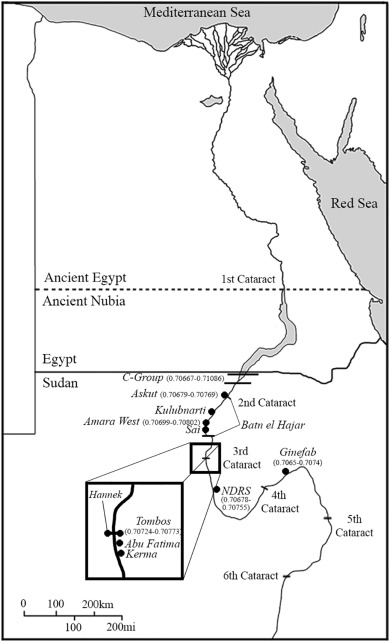
\includegraphics[width=0.35\textwidth]{egypt_regions.jpg}
    \caption{A map of Egypt, with the regions under study highlighted \citep{schrader2019}. }
    \label{fig:egypt_regions}
\end{figure}

Accounts of ancient Egyptians are incomplete because of they lived long ago.
\cite{schrader2019} sought to investigate the movement of rural and urban settlements
in the Third Nile Cataract region of Egypt from 2500 BCE to 656 BCE.

To achieve this, the researchers measured strontium isotope ratios of tooth enamel samples to
identify local and non-local skeletons in three Egyptian graveyards, which range
across time and urbanness.

The researchers concluded that, across the board, there were numerous non-local
people alongside local people. And, all of the non-local strontium ratios were higher than the local ones.
They reason that this indicates migraiton between the Second and Third
Nile Cataract was normal in ancient times. This is enforced by the fact that
even skeletons in ostensibly poorer graveyards showed non-local people, which likely
means that people across financial brackets migrated consistently.

% - 2500 BCE - 656 BCE
% - Figuring out mobility of rural and urban settlements in Egypt over time
% - Methods:
% --> Dental Sr to determine localness of Abu Fatima, Hannek, and Tombos graves
% - Conclusions:
% --> Across the board, there were some non-local people, which indicates that migration was normal b/w First and Second Nile Cataract
% --> Even poorer people migrated



% \citep{schrader2019} https://www.sciencedirect.com/science/article/pii/S2352409X18305509?casa_token=5XDdWMPYLpEAAAAA:YAvhcSklHzL7SZB_V2M3eqXaZK8AzFKP4Iw3pTXD0Opp1u-KSGONBW4X3lEHp5sc62fgnhWs0oU#s0015

% \section{Conclusion}
% Strontium isotope analysis is a relevant and useful tool for archeologists studying
% Ancient Egypt. Strontium isotope analysis involves measuring the ratio of
% \textsuperscript{87}Sr and \textsuperscript{86}Sr in humans, plants, and animals, which
% is generally unique across geographic areas.

% This tool has clear applications for questions of provenance, or place of origin.
% Researchers can measure the strontium ratios in organic matter and then compare this ratio
% to nearby environmental ratios measured beforehand to pinpoint what geographic region
% the organic matter formed in. Since tooth enamel in humans form during childhood,
% researcheres can figure out where the human lived during their childhood.

% Recently, strontium isotope analysis has exploded in popularity for
% its utility in ascertaining provenance. Archeologists have increasingly taken
% advantage of this method to answer questions
% ranging from power rises to ancient economies to migrational patterns.
% Strontium isotope analysis will only become more relevant as time goes on. Thus,
% I encourage all archeological researchers to learn what it is and find out how to apply
% it to answer their research questions.
\section{Conclusion}
In conclusion, strontium isotope analysis emerges as a potent and illuminating
tool for delving into the mysteries of Ancient Egypt. The method, which
discerns the geographic origins of humans and animals through the examination of
strontium isotope ratios in their remains, provides a unique lens into the past.

Through this paper, I've explored the foundations and applications of strontium
isotope analysis, particularly in the context of Ancient Egypt. Strontium isotope
analysis reveals the historical mobility and migration patterns of ancient
populations, challenging conventional narratives and shedding light on the
dynamic nature of human societies.

Case studies, such as the investigation into the origins of the Hyksos and the
migrational patterns in ancient Egypt, exemplify the method's capacity to
rewrite historical interpretations. The ability to discern the provenance of
individuals, animals, and even crops enhances our understanding of trade,
societal structures, and environmental interactions.

Beyond the realm of archaeology, strontium isotope analysis extends its utility
to diverse fields. From forensics, where it aids in post-mortem investigations,
to conservation efforts by tracking the illegal trade of animal products, this
analytical method demonstrates its versatility and relevance.

The study of mummified birds and the assessment of migrational origins in
Ancient Egypt showcase the breadth of insights that strontium isotope analysis
can provide. Despite its strengths, strontium isotope analysis is not without
limitations. Challenges related to precision, accuracy, and cost underscore the
need for a nuanced approach and complementary methods.

However, ongoing advancements in technology and analytical techniques hold the
promise of overcoming these challenges, making strontium isotope analysis an
increasingly indispensable tool in the archaeologist's toolkit. As our
understanding of strontium isotope analysis continues to evolve, it opens
avenues for interdisciplinary research, encouraging collaboration between
archaeologists, chemists, and environmental scientists.

By unraveling the secrets embedded in skeletal remains and ancient artifacts,
strontium isotope analysis contributes significantly to reconstructing the
intricate tapestry of human history. In conclusion, the journey through the
survey of strontium isotope analysis in archaeological research of Ancient Egypt
underscores its significance in unraveling the complexities of the past,
paving the way for a more nuanced and enriched narrative of human civilization.

\section{Acknowledgment}

This article was partially generated with assistance from ChatGPT, an OpenAI language model.


% Bibliography
\bibliographystyle{apalike}
\bibliography{references} % Specify your bibliography file (e.g., references.bib)

\end{document}
